\documentclass[border=3pt,tikz]{standalone}
\usepackage{amsmath}
\begin{document}
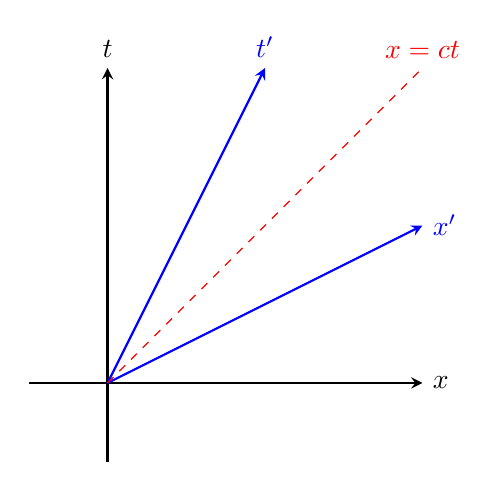
\begin{tikzpicture}[]
    \draw[thick,->,>=stealth] (0, -1) -- (0, 4) node[above] {$t$};
    \draw[thick,->,>=stealth] (-1, 0) -- (4, 0) node[right] {$x$};
    \draw[thick, blue, ->,>=stealth] (0,0)-- (2, 4) node[above] {$t^\prime$};
    \draw[thick, blue, ->,>=stealth] (0,0)-- (4, 2) node[right] {$x^\prime$};
    \draw[red, dashed] (0,0)-- (4, 4) node[above] {$x=ct$};
    \end{tikzpicture}
\end{document}